\section{Solution}
In this section we describe the key ideas behind our design, and the decisions we made during the design process.
\subsection{Idea}

Figure ~\ref{fig:architecture} shows an architecture diagram of our design.

To store the last 4 input values for each of the streams,  we allocate 4 arrays of size $n$ in BRAM. When input is ready we move the contents of the $i^{th}$ array to the $(i+1)^{th}$ for $0 \leq i < 4$, and store the input value corresponding to $j{th}$ stream to the $j^{th}$ block of array 0. The filtering happens as follows. For $0 \leq  i < n$ and $0 \leq j < 4$ we load the $i^{th}$ value from the $j^{th}$ array from the input buffer arrays.  These 4 values are used as input values for the FIR, together with the corresponding coefficients according to the direct equation for the filter. The values from the array are requested one clock cycle before they are needed in the computation, since reads in the BRAM are performed synchronously. As seen in the diagram, we use 4 multipliers in parallel. Alternatively we could have used one multiplier doing 4 sequential operations for each sample, but we decided to optimize for throughput and not for hardware usage.

The coefficients $h[]$ are the same as in lab L4 and because they are symmetric we store only $2L+1$ of them.

The input storing and FIR processing for each stream happens in the same clock cycle, so that we could theoretically produce one output per clock cycle.
\begin{figure}
\begin{center}
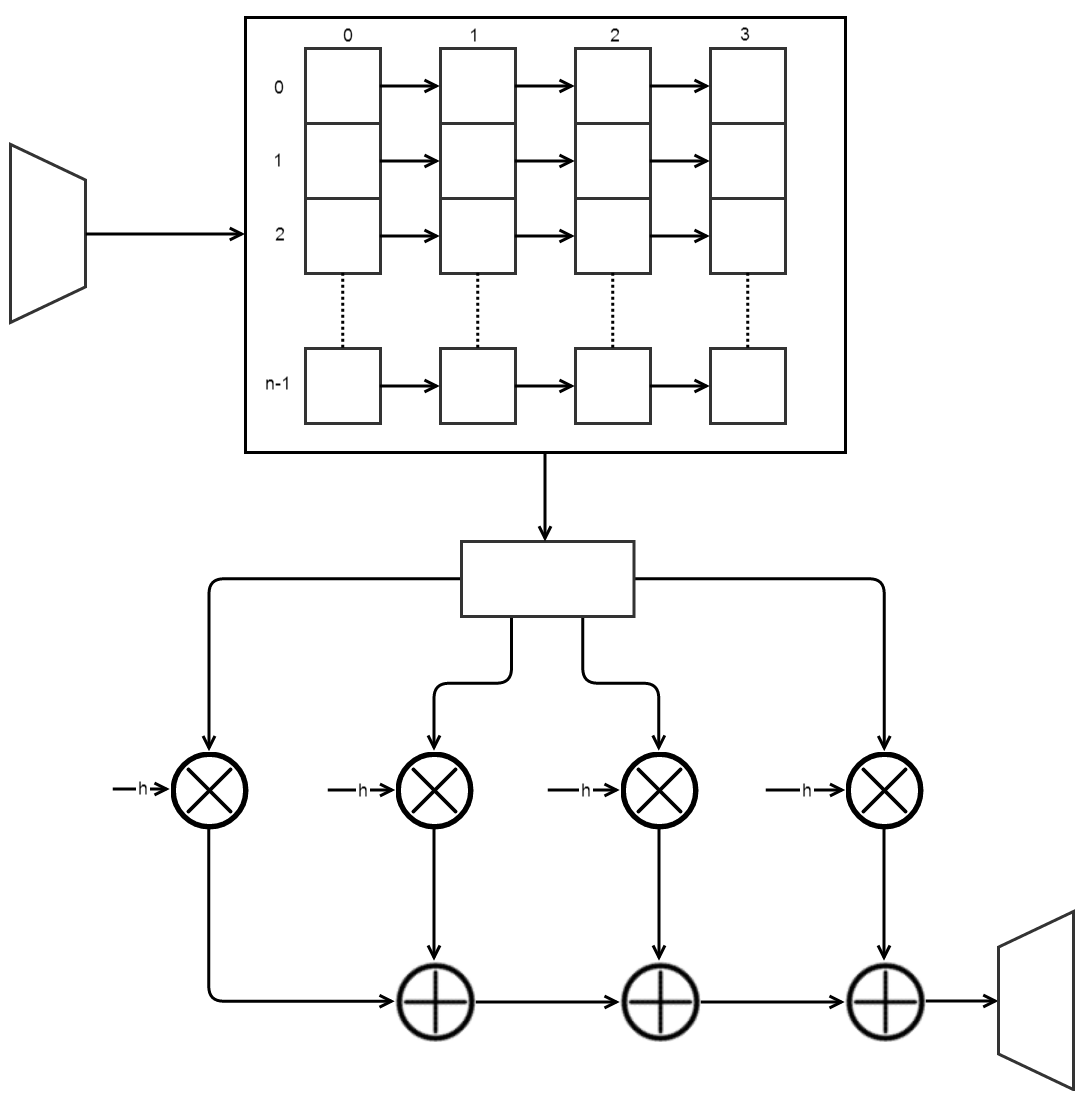
\includegraphics[width=0.7\textwidth]{images/architecture.png}
\caption{Architecture diagram of the system.}
\label{fig:architecture}
\end{center}
\end{figure}
\FloatBarrier
\subsection{Implementation}
In this section we will explain functional correctness of our code. The Verilog source code of our filter can be found in section ~\ref{sec:source}. \\
\\
\centerline{reg [0:NR\_STREAMS\_LOG-1] stream;}\\
\\
We have 1024 streams. This register hold the index of the stream we are currently processing.\\
\\
\centerline{reg [0:L\_LOG-1] l;}\\
\\
We use the direct equation, this register store the value of $nM \bmod L$, so we can calculate it using only conditionals and adders.\\
\\
\centerline{reg [0:L\_LOG-1] m;}\\
\\
Holds a delayed value of $l$, this is required to compensate for the fact that I/O and computation happen simultaneously.\\
\\
\centerline{reg signed [0:DDWIDTH-1] in0 [0:NR\_STREAMS-1];}\\
\centerline{reg signed [0:DDWIDTH-1] in1 [0:NR\_STREAMS-1];}\\
\centerline{reg signed [0:DDWIDTH-1] in2 [0:NR\_STREAMS-1];}\\
\centerline{reg signed [0:DDWIDTH-1] in3 [0:NR\_STREAMS-1];}\\
\\
We need to store the 4 latest values of all 1024 input streams.\\
\\
\centerline{reg signed [0:DWIDTH-1] h [0:2*L];}\\
\\
We need to store our coefficients. The coefficients are symmetric, so we can do an optimization storing only $2L + 1$ coefficients.\\
\\
\centerline{\$readmemh("coefficients.txt", h);}\\
\\
Our coefficients are read from a file. These values are precalculated by a small Java program.\\
\begin{center}
\parbox{10cm}{
in0[stream] $<=$ data\_in;\\
in1[stream] $<=$ in0[stream];\\
in2[stream] $<=$ in1[stream];\\
in3[stream] $<=$ in2[stream];\\
req\_out\_buf $<=$ 0;\\
}
\end{center}
As seen in figure ~\ref{fig:arch}, all values in the input buffer are shifted, the new input is loaded into the first.\\
\begin{center}
\parbox{10cm}{
if( l $<$ L - M )\\
begin\\
\phantom{xxxx} l $<=$ l + M;\\
end\\
else\\
begin\\
\phantom{xxxx}l $<=$ l - (L - M);\\
\phantom{xxxx}req\_in\_buf $<=$ 1;\\
end\\
}
\end{center}
This is used to efficiently calculate the value of $(l + M) \bmod L$. Instead of applying the $\bmod$ operation each time, we store the value, and increment in by $l + M$. When this value becomes larger or equal to  $L - M$ we have to subtract $L - M$.\\
\begin{center}
\parbox{10cm}{
sum $<=$ in0[stream] * h[m] + in1[stream] * h[m+L] + in2[stream] * h[L*2-m] + in3[stream] * h[L-m];
}
\end{center}
This is the filtering part, we have 4 multiplications and 3 additions.
